\documentclass[12pt]{article}
\usepackage{a4wide, amsfonts, epsfig,bbding,phonetic}

\begin{document}
\begin{center}
{\bf EMAT10001 Lecture 17.}\\[1cm]{} Conor Houghton 2014-2-23
\end{center}
\subsection*{Preface} 
These are outline notes for lecture 16. As usual there is a bounty of
between 20p and \pounds 2 for errors, you can tell me at the end of a
lecture or email me at \texttt{conor.houghton{@}bristol.ac.uk}.

\subsection*{Introduction}

This is a lecture about the Fourier series and the Fourier transform.

\subsection*{Vector spaces and inner product spaces}

We are familiar with vectors, things like $\mathbf{v}$. If
$\mathbf{u}$ and $\mathbf{v}$ are two vectors we can add them
$\mathbf{u}+\mathbf{v}$:
\begin{center}
\setlength{\unitlength}{4144sp}%
%
\begingroup\makeatletter\ifx\SetFigFont\undefined%
\gdef\SetFigFont#1#2#3#4#5{%
  \reset@font\fontsize{#1}{#2pt}%
  \fontfamily{#3}\fontseries{#4}\fontshape{#5}%
  \selectfont}%
\fi\endgroup%
\begin{picture}(1512,972)(2236,-3901)
\thinlines
{\put(2501,-3886){\vector( 3, 1){1215}}
}%
{\put(3691,-3481){\vector(-4, 3){720}}
}%
{\put(2501,-3881){\vector( 1, 2){470}}
}%
\put(3286,-3886){\makebox(0,0)[lb]{\smash{{\SetFigFont{12}{14.4}{\rmdefault}{\mddefault}{\updefault}{$\mathbf{u}$}%
}}}}
\put(3421,-3076){\makebox(0,0)[lb]{\smash{{\SetFigFont{12}{14.4}{\rmdefault}{\mddefault}{\updefault}{$\mathbf{v}$}%
}}}}
\put(2251,-3301){\makebox(0,0)[lb]{\smash{{\SetFigFont{12}{14.4}{\rmdefault}{\mddefault}{\updefault}{$\mathbf{u+v}$}%
}}}}
\end{picture}%
\end{center}
We can multiply vectors by scalars, ordinary numbers, so if we have
$\mathbf{u}$ and $a$ then $a\mathbf{u}$ is the vector which points in
the same direction as $\mathbf{u}$ but is $a$ times longer. We also
have the \textsl{dot product}, 
\begin{equation}
\mathbf{u}\cdot\mathbf{v}=|\mathbf{u}||\mathbf{v}|\cos{\theta}
\end{equation}

Just like symmetry is abstracted away to give groups, there is a
mathematical structure called a \textsl{vector space} for a set of
objects that have addition and scalar multiplication and with some
property to demand that the addition and scalar multiplication behave
nicely, we won't go through these now but they are things like
$(a+b)\mathbf{u}=a\mathbf{u}+b\mathbf{u}$. Some vector spaces are
inner product spaces if there is an \textsl{inner product}, that is a
map that sends pairs of vectors to a number, just like the \textsl{dot
  product} does. Again, there are niceness properties, like 
\begin{equation}
(\mathbf{u}+\mathbf{v})\cdot\mathbf{w}=\mathbf{u}\cdot\mathbf{w}+\mathbf{v}\cdot\mathbf{w}
\end{equation}
and
\begin{equation}
\mathbf{u}\cdot\mathbf{v}=\mathbf{v}\cdot\mathbf{u}
\end{equation}
Anyway, the key point is that the dot product is an example of such a
thing. Furthermore, if you have a inner product, you have a
\textsl{norm}, a way of measuring length
\begin{equation}
|\mathbf{u}|=\sqrt{\mathbf{u}\cdot\mathbf{u}}
\end{equation}

The reason we mention this is that being an inner product space allows
you to convert between two ways of thinking about vectors, the
original way, as something with a length and a direction, and the
component form, things like $\mathbf{u}=(u_1,u_2,u_3)$. The story goes
like this, it is possible to find independent unit length orthogonal
vectors, in three dimensions these are often taken to be the three
vectors $\mathbf{i}$, $\mathbf{j}$ and $\mathbf{k}$ where 
\begin{equation}
|\mathbf{i}|=|\mathbf{j}|=|\mathbf{k}|=1
\end{equation}
and
\begin{equation}
\mathbf{i}\cdot\mathbf{j}=0
\end{equation}
and so on. Now, if we are in three dimensions and we have three of
these vectors, we are able to write any other vector in terms of them
\begin{equation}
\mathbf{u}=u_1\mathbf{i}+u_2\mathbf{j}+u_3\mathbf{k}
\end{equation}
Now try dot producting both sides with $\mathbf{i}$
\begin{equation}
\mathbf{u}\cdot\mathbf{i}=u_1\mathbf{i}\cdot\mathbf{i}+u_2\mathbf{j}\cdot\mathbf{i}+u_3\mathbf{k}\cdot\mathbf{i}=u_1
\end{equation}
In other words
\begin{equation}
u_1=\mathbf{u}\cdot\mathbf{i}
\end{equation}
Similarly $u_2=\mathbf{u}\cdot\mathbf{j}$ and
$u_3=\mathbf{u}\cdot\mathbf{k}$. Hence, if we are in an inner product
space we can work out components $(u_1,u_2,u_3)$ where $u_1$ is the
projection in the $\mathbf{i}$-direction, and so on. 

\subsection*{Fourier series}
The amazing thing is that the space of functions is also an inner
product space. Lets first of all think about periodic function and for
simplicity we are going to imagine the period is $2\pi$. Hence, we are thinking about functions $f(t)$ such that
\begin{equation}
f(t+2\pi)=f(t)
\end{equation}
Now this is a vector space, if $f(t)$ and $g(t)$ are both functions with period $2\pi$ so is $h(t)=f(t)+g(t)$:
\begin{equation}
h(t+2\pi)=f(t+2\pi)+g(t+2\pi)=f(t)+g(t)=h(t)
\end{equation}
and, if $af(t)$ is a periodic function with period $2\pi$ if $f(t)$
is. 

It is also an inner product space, though this might be less obvious,
but given two periodic functions $f(t)$ and $g(t)$ an inner product is
given by
\begin{equation}
(f,g)=\frac{1}{\pi}\int_{-\pi}^\pi f(t)g(t)dt
\end{equation}
Don't worry about the $1/\pi$, it is just there to make some formulas
later look neater, the basic point is that there is a way of going
from two of these functions to a scalar and, though we haven't listed
them, it does turn out that this satisfies all the required niceness
properties.

So, the space of periodic functions is an inner product space. This is
nice to know since it means we can now start seeing if stuff that
works with vectors works with periodic functions. The obvious thing to
try is the splitting up into components that worked so well with
vectors. Thus, the question is, is there a set of basic functions like
the basis vectors $\mathbf{i}$, $\mathbf{j}$ and $\mathbf{k}$? The
answer is yes, they are sine and cosines. In fact
\begin{eqnarray}
\frac{1}{\pi}\int_{-\pi}^\pi \sin{nt}\sin{mt}dt&=&\delta_{nm}\cr
\frac{1}{\pi}\int_{-\pi}^\pi \sin{nt}\cos{mt}dt&=&0\cr
\frac{1}{\pi}\int_{-\pi}^\pi \cos{nt}\cos{mt}dt&=&\delta_{nm}
\end{eqnarray}
where $\delta_{nm}$ is the Kronecker $\delta$-function which is one if $n$ and $m$ are equal, and zero if they aren't
\begin{equation}
\delta_{nm}=\left\{\begin{array}{ll}1&n=m\\0&\mbox{otherwise}\end{array}\right.
\end{equation}
So, it looks a little confusing since we have two different types of
basis functions, but sine and cosines have the same sort of
orthogonality relationship that the $\mathbf{i}$, $\mathbf{j}$ and
$\mathbf{k}$ had. In fact, to make it even more confusing for there to
be enough basis vectors we have to include the possibility that $n=0$
for the cosines, giving just a constant, and the normalization is
different for the constant. However, the net effect is we can
decompose periodic functions just like we can ordinary vectors.

So, in short, we can write
\begin{equation}
f(t)=\frac{1}{2}a_0+\sum_{n=1}^\infty{a_n\cos{n t}}+\sum_{n=1}^\infty{b_n\sin{n t}}
\end{equation}
We haven't, in a sense, proven that we have enough basis vectors for
this to work, and that's actually very tricky to prove, but assuming
there are we can work out the $a_n$ and $b_n$ the same way we did for
$u_1$ and so on. For example, for $a_n$ with $n\not=0$ multiply both
side by $\cos{mt}$ and integrate
\begin{eqnarray}
\frac{1}{\pi}\int_{-\pi}^\pi \cos{mt}f(t)dt&=&\frac{1}{2}a_0\frac{1}{\pi}\int_{-\pi}^\pi\cos{mt}dt +\sum_{n=1}^\infty{a_n\frac{1}{\pi}\int_{-\pi}^\pi \cos{mt}\cos{n t}dt}\cr
&&+\sum_{n=1}^\infty{b_n\frac{1}{\pi}\int_{-\pi}^\pi \cos{mt}\sin{n t}dt}
\end{eqnarray}
then, since almost everything is zero, we end up with
\begin{equation}
a_m=\frac{1}{\pi}\int_{-\pi}^\pi \cos{mt}f(t)dt
\end{equation}
so this is like the projection of $f(t)$ onto $\cos{mt}$. Doing the
same thing with sine and with just straight integration of both sides
we get
\begin{eqnarray}
a_0&=&\frac{1}{\pi}\int_{-\pi}^{\pi}f(t)dt\cr
a_n&=&\frac{1}{\pi}\int_{-\pi}^{\pi}f(t)\cos{n t}dt\cr
b_n&=&\frac{1}{\pi}\int_{-\pi}^{\pi}f(t)\sin{n t}dt
\end{eqnarray} 
This is the Fourier series.

\subsection*{Example} 
Consider the block wave with period $2\pi$
\begin{equation}
f(t)=\left\{\begin{array}{ll}1&0<t<\pi\\-1&-\pi<t<0\end{array}\right.
\end{equation}
with $f(t+2\pi)=f(t)$.
\begin{center}
\begin{picture}(170,120)(35,580)
\thinlines
\put( 15,620){\line( 1, 0){200}}
\put( 110,660){\line( 0,-1){ 80}}
\put( 110,650){\line( 1,0){ 40}}
\put( 150,590){\line( 1,0){ 40}}
\put( 190,620){\line( 0,-1){ 3}}
\put( 150,620){\line( 0,-1){ 3}}
\put( 110,620){\line( 0,-1){ 3}}
\put(  70,620){\line( 0,-1){ 3}}
\put(  30,620){\line( 0,-1){ 3}}
\put( 190,650){\line( 1,0){ 25}}
\put( 218,650){\line( 1,0){  2}}
\put( 223,650){\line( 1,0){  2}}
\put( 228,650){\line( 1,0){  2}}
\put(  70,590){\line( 1,0){ 40}}
\put(  30,650){\line( 1,0){ 40}}
\put(  15,590){\line( 1,0){ 15}}
\put(  10,590){\line( 1,0){  2}}
\put(   5,590){\line( 1,0){  2}}
\put(   0,590){\line( 1,0){  2}}
\put( 100,646){\makebox(0,0)[lb]{1}}
\put( 115,587){\makebox(0,0)[lb]{-1}}
\put(  20,607){\makebox(0,0)[lb]{$-2\pi$}}
\put(  60,607){\makebox(0,0)[lb]{$-\pi$}}
\put( 145,607){\makebox(0,0)[lb]{$\pi$}}
\put( 185,607){\makebox(0,0)[lb]{$2\pi$}}
\end{picture}
\end{center}
So
\begin{equation}
a_n=\frac{1}{\pi}\int_{-\pi}^{\pi} f(t)\cos{nt}dt
\end{equation}
Since $f(t)$ is \textsl{odd}, that is $f(t)=-f(-t)$, this can be shown
to be zero by a standard trick. Let $t'=-t$ and do a change of
variable in the integral: $dt'=-dt$ but when $t=\pi$, $t'=-\pi$ and
visa versa; flipping the limits around gives an extra minus, so
\begin{equation}
a_n=\frac{1}{\pi}\int_{-\pi}^{\pi}f(t)\cos{nt}dt=\frac{1}{\pi}\int_{-\pi}^{\pi} f(-t')\cos{(-nt')}dt'=-\frac{1}{\pi}\int_{-\pi}^{\pi}f(t')\cos{(nt')}dt'=-a_n
\end{equation}
and, if $a_n=-a_n$ then it must be zero. A similar trick works for
$b_n$ is the function is even, that is, if $f(t)=f(-t)$. In this way
$a_n$ is thought of as dealing with the even part of the function and
$b_n$ with the odd part.

As for the $b_n$, you need to do this by integration
\begin{equation}
b_n=\frac{1}{\pi}\int_{-\pi}^{\pi}dt f(t)\sin{nt}=\frac{2}{\pi}\int_0^{\pi}dt \sin{nt}=-\left.\frac{2\cos{nt}}{n\pi}\right|_0^\pi=\frac{2}{\pi n}[1-(-1)^n]
\end{equation}
where we have used $\cos{n\pi}=(-1)^n$. Hence
\begin{equation}
f(t)=\frac{4}{\pi}\sum_{n\mbox{\,{\scriptsize odd}}}{\frac{1}{n}\sin{nt}}
\end{equation}

If we write
\begin{equation}
f_N(t)=\frac{4}{\pi}\sum_{n\mbox{ {\scriptsize odd,} }n\le N}\frac{1}{n}\sin{nt}
\end{equation}
then
\begin{center}
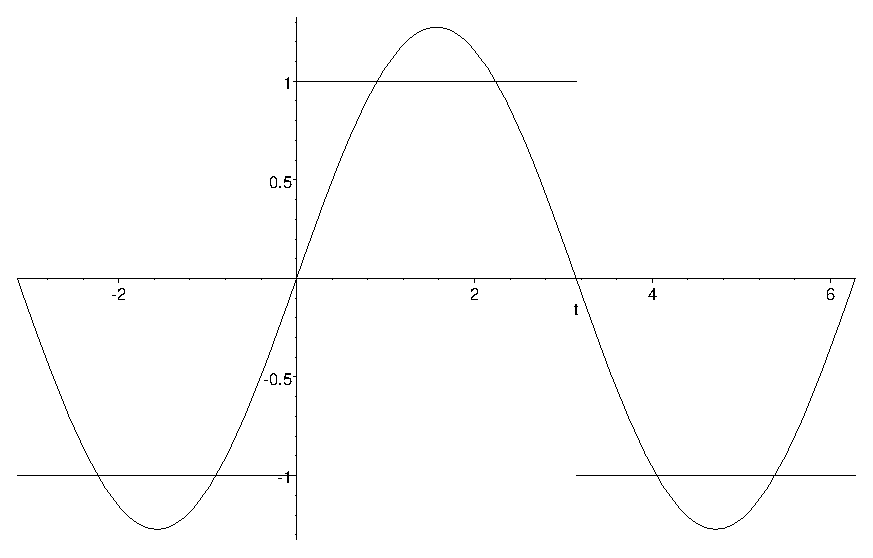
\epsfig{file=1.eps,width=8cm}
$f_1(t)$
\end{center}

\begin{center}
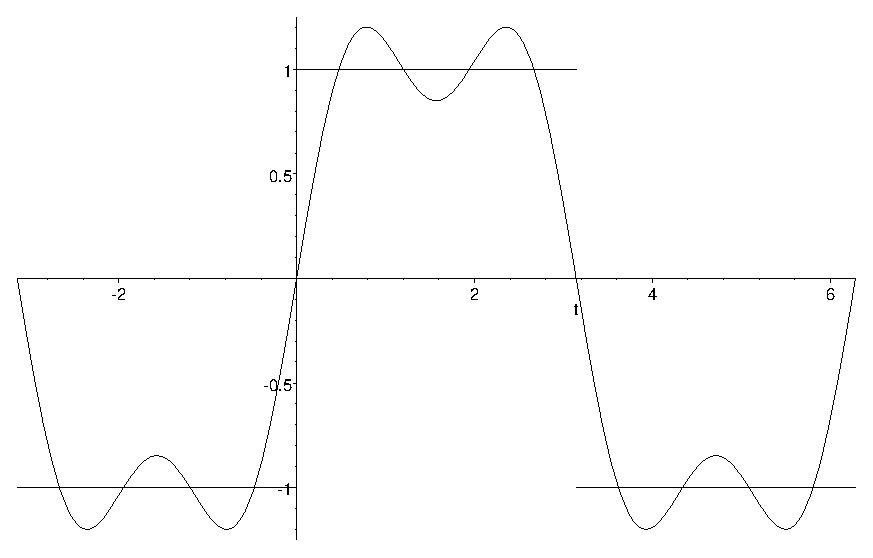
\epsfig{file=3.eps,width=8cm}
$f_3(t)$
\end{center}


\begin{center}
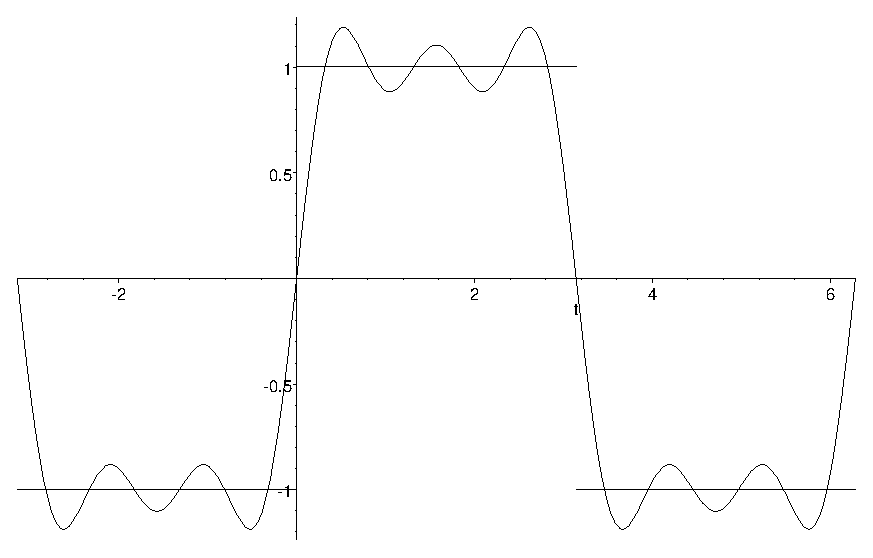
\epsfig{file=5.eps,width=8cm}
$f_5(t)$
\end{center}


\begin{center}
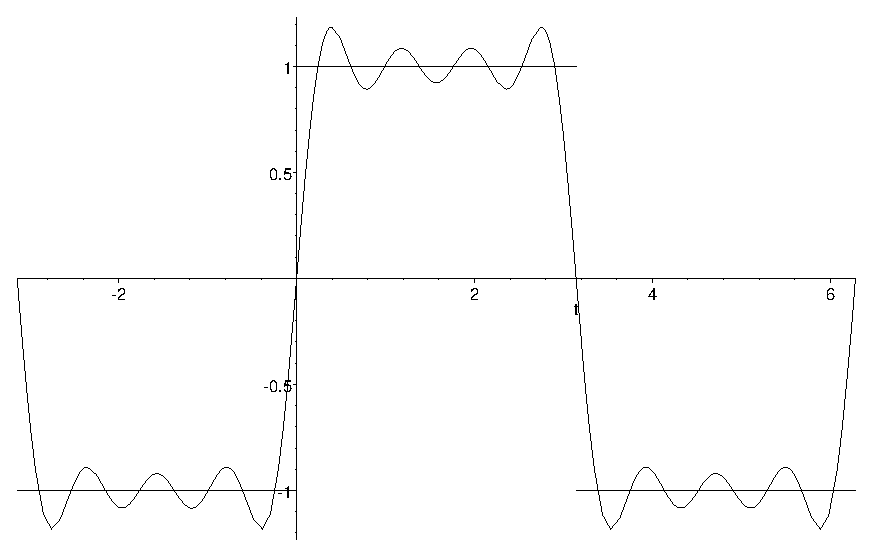
\epsfig{file=7.eps,width=8cm}
$f_7(t)$
\end{center}


\begin{center}
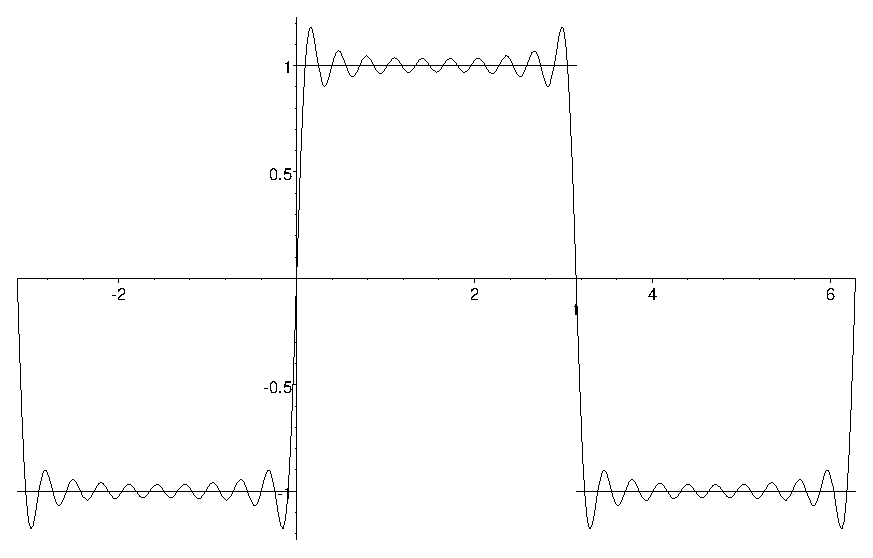
\epsfig{file=19.eps,width=8cm}
$f_{19}(t)$
\end{center}

In fact, this is a very artificial example, not at all like the
examples that arise in image processing. It is commonly looked at only
because the integration is relatively easy to do. In real examples the
integration can't be done explicitely, but there is an extremely
powerful numerical technique called the Fast Fourier Transform.

\subsection*{Application}

This might all seem a bit odd, but, in fact, the Fourier series has
many applications. Basically what is happening in a Fourier series is
that we are replacing a picture of the function that looks at the
value of the function at different values of $t$ with a picture that
looks at how much of the function can be explained by different sines
and cosines. Since the sines and cosines get wavier at higher and
higher $n$ then the size of $a_n$ and $b_n$ describes how much of the
detail of the function is found at a length scale of $2\pi/n$.

One common computer science or electronic engineering application of
Fourier series is cleaning up or compressing a signal. For example,
for sound, if you convert a sound wave into its Fourier series and
then truncate it so that you leave out values of $n$ that correspond
to frequencies humans can't hear, the sound will be described in a
more compressed way, but without any loss in how the sound is
heard. Common video compression methods, like mpeg, work like this;
they are cleverer in that they not only drop the high frequencies that
we can't hear, the also take into account masking, an auditory effect
were if some $a_n$ and $b_n$s are large you can set the smaller ones
to zero without affecting sound quality. Other compression methods use
a similar approach, but replace the sines and cosines with other basis
sets.

Another application relates to sampling. Typically a signal is known
only from a discrete sampling, a sound wave may be measured at
discrete points in time, for example. It is useful to reconstruct the
signal, but this can't be done at a level of detail that excedes the
sampling rate, basically the reconstructed signal is like the
truncated Fourier series, leaving out $a_n$ and $b_n$s for the $n$s
where the detail probed by the corresponding $\sin{nt}$ and $\cos{nt}$
is smaller than the gap between the sample points. This is dealt with
in a theorem called the Shannon-Nyquist sampling theorem.

In Fourier series also has many applications in mathematical physics,
there are equations, like the heat equation, that can only be solved
using Fourier methods and quantum mechanics is usually formulated in a
way that hops between the original $f(t)$-style perspective of a
function and a perspective based on the Fourier approach.

We have been looking specifically at functions with period $2\pi$;
this can easily be generalized to other periods. Another change is to
replace the sines and cosines with $\exp(int)=\cos{nt}+i\sin{nt}$,
this looks more annoying at first since it includes complex numbers,
but it turns out to be more elegant. A bigger change is to consider
non-periodic functions, a similar approach works provided they decay
rapidly to zero for large $|t|$, however in this case just looking at
$\cos{nt}$ and $\sin{nt}$ for integer $n$ does not give enough basis
functions, you need to use a continuous set of basis functions, this
leads to the Fourier transform
\begin{eqnarray}
f(t)&=&\int_{-\infty}^{\infty}dk\,\widetilde{f(k)}e^{ikt}\cr
\widetilde{f(k)}&=&\frac{1}{2\pi}\int_{-\infty}^{\infty}dt\,f(t)e^{-ikt}
\end{eqnarray}
where a real number $k$ have replaced the $n$, an integral has
replaced the sum and $\widetilde{f(k)}$ has replaced the $a_n$ and
$b_n$. In fact, in practice, we use a mixture of Fourier series,
Fourier transform, and windowed Fourier transforms, where you look at
the little bit of the original signal at a time and do a Fourier
transform on that.





\end{document}

